\section{Proactive Approaches}
Proactive approaches aim at lowering the possibility of Tor users being affected by an active BGP routing attack. Network-level adversaries can announce a more-specific prefix or an equally-specific prefix to hijack the traffic between the client and the Tor guard relay. To counter these routing attacks, we propose two methods: 1) convincing relay operators to announce the relay in a /24 prefix to defend against a more-specific prefix hijack attack, and 2) introducing a new Tor guard relay selection algorithm that minimizes the likelihood that a Tor client sees a hijacked route in the case of an equally-specific prefix hijack attack.

\subsection{Using /24 Prefixes}
\label{subsec:24prefix}

Sun \emph{et al.} \cite{sun2015raptor} recently found that more than 90\% of BGP prefixes hosting relays are
shorter than /24, making them vulnerable to a more-specific BGP prefix attack. We measured the distribution of prefix lengths in relation to Tor bandwidth using the Tor consensus data in January 2016; this is shown in ~\ref{fig_prefixlen}. Consistent with the findings in \cite{sun2015raptor}, a large percentage of the bandwidth are under prefixes shorter than /24. Thus, one quick way to make Tor relays more resilient to such active routing attacks is to announce a /24 prefix covering each Tor relay. In order to make real world impact of this approach, we start a campaign by contacting network operators whose prefixes contain Tor relays, and asking them to announce a more specific /24 prefix covering the relay. 

\begin{figure}[ht!]
\centering
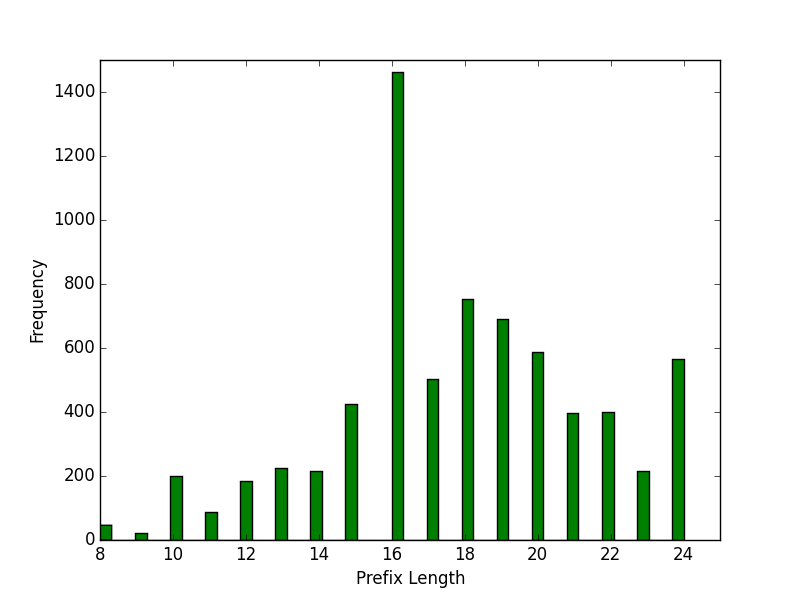
\includegraphics[width=80mm]{prefix_len_graph}
\caption{Distribution of Tor bandwidth to Prefix Lengths \yixin{we need to fix this plot} \label{fig_prefixlen}}
\end{figure}

We start by cooperating with Princeton University, which contains a Tor relay under a /16 prefix. 

\subsection{Guard Relay Selection}
\label{subsec:relayselection}

Guard relays are at an important position in the Tor circuit, since they have direct connections with Tor clients. It has been shown that network-level adversaries can launch a more-specific BGP prefix hijack attack to hijack the Tor traffic from the guard relay to the malicious AS \cite{sun2015raptor}. This can be potentially prevented by advertising /24 prefixes, as discussed in Section \ref{subsec:24prefix}. However, even if the guard relay belongs to a /24 prefix, it is still susceptible to an equally-specific prefix attack. Unlike more-specific attacks which spread through the whole Internet, equally-specific attacks can only affect connections within a small range - i.e., ASes that have more preferred paths to the hijacking AS than the true origin AS. Thus, picking a Tor guard relay that has relatively high AS resilience against such equally-specific attacks could protect Tor clients from being affected and deanonymized by network-level adversaries. Therefore, we propose a new guard relay selection algorithm that incorporates resilience.

\subsubsection{Design Goals}
\begin{enumerate}
\item \emph{Mitigate prefix hijacks on Tor.} This is the main goal of the new guard relay selection algorithm. The algorithm computes the AS resilience against prefix hijacks of all Tor guard relays from the client's AS, and prefers the ones that have higher resilience, minimizing the likelihood that the client would be affected by a prefix hijack on its guard relay. 
\item \emph{Protect the anonymity and privacy of Tor clients.} In addition to lowering possibilities of being hijacked, the algorithm should also protect the anonymity of Tor users, i.e., variance in relay selection preferences and sender/recipient anonymity. 
\item \emph{Load balance Tor traffic.} The algorithm should incorporate relay bandwidth into selection decision and avoid causing excessive traffic congestion on low bandwidth relays. 
\item \emph{Performance overhead.} The algorithm should have a reasonable performance overhead over the vanilla Tor algorithm when bootstrapping, and fast page load time. 
\end{enumerate}

\subsubsection{Deal with the possibility of prefix hijacks}

In section ~\ref{hijack_methodology}, we measured AS resilience of each Tor-related AS based on the metrics proposed by~\cite{lad2007understanding}. The algorithm computes \emph{total} resilience of an AS by summing individual resiliencies from each source AS. \emph{However, the Tor client would only care about the individual resilience to a Tor-related AS from the source AS where the client is located}. Thus, instead of computing the total resilience, we use Algorithm ~\ref{algo:calcres} to calculate resilience $R(i)$ of each Tor-related AS $i$, from the client AS $t$. 

Tor relay selection is bandwidth-aware and prefers high bandwidth relays. The probability of each relay $i$ being chosen is based on its bandwidth $B(i)$. Thus, in order to still provide clients with the load balancing option of Tor bandwidths, we offer a tunable parameter $\alpha$ in the relay selection algorithm combining AS resiliency $R(i)$ and bandwidth $B(i)$. Each relay $i$ will be assigned a weight as following:
\begin{equation*}
W(i) = \alpha \times R(i) + (1 - \alpha) \times B(i)
\end{equation*}
Note that, when $\alpha$ is set to $0$, the relay selection becomes the same as bandwidth-only selection; while when $\alpha$ is set to $1$, the selection becomes resiliency-only selection. 

\subsubsection{Randomization is needed}

If we simply select the set of guard relays based on the probability of $relay\_weight/total\_weight$, an adversary can potentially run a relay that has a short AS-level path to the Tor client, such that it has high resilience from the client AS, and thus obtains high probability of being chosen. Furthermore, the Tor client might also be susceptible to fingerprinting attacks due to the differences in relay selection probabilities based on AS-location of the client. An adversary that can observe the client for a long enough time may be able to infer the AS-location of the client based on its observed relay selection choices. Thus, we need to take into account these potential vulnerabilities and protect the anonymity of clients. Note that, the weight of a Tor relay depends on two factors: (1) resilience of the AS where the relay is located, and (2) the relay's bandwidth. The relay's bandwidth is not specific to client locations, and thus would not reveal any client identities; in addition, it is not trivial to run a high bandwidth relay with significantly higher bandwidth than all other relays to obtain high probability of being chosen due to resource constraints. While on the contrary, AS resilience of relays \emph{is} client-specific, and requires much less resources to run a malicious relay with high AS resilience.

Instead of using resilience $R(i)$ for relay $i$ directly in the weight calculation, we first adjust it to $R(i)\prime$ by performing a pseudorandom sampling without replacement using an algorithm proposed by Tille \yixin{(cite here)}. We compute the inclusion probability of each relay $i$ into a sample of size $(g \cdot total\_TorASes)$ given the fraction of its resilience $R(i)$ over total resilience $\sum R(i)$.  Then divide the inclusion probability by sample size $(g \cdot total\_TorASes)$ to get the probability of being chosen randomly within the sample. Thus, the new resilience weight becomes:

\begin{equation*}
R(i) \prime = \frac {\pi(i | (g \cdot N))} {g \cdot N}
\end{equation*}

in which $\pi(i | m)$ represents the inclusion probability of relay $i$ given sample size $m$, where $N$ is the total number of ASes in which Tor relays reside. $g$ is a configurable parameter indicating the percentage of random sampling we want to perform in the Tor-related AS set. Note that when $g$ is set to $0$, then no random sampling will be performed, while if $g$ is set to $1$, then all relays will have the same $R(i)\prime$ in their weights.

%Instead of selecting relay directly based on its weight, we will first select a cluster of 
%\begin{equation*}
%m + \alpha \cdot g \cdot (N - m)
%\end{equation*}
%number of relays, in which $m$ is the minimum number of relays needed (i.e., 1 for single guard and 3 for multiple guards), $N$ is the total number of relays and $g$ is a configurable parameter indicating the maximum percentage of additional relays we want to pick into the cluster. Then, we will pick the guard relay(s) at random from the cluster. Note that when $g$ is set to $0$, then no additional randomization will be performed, while if $g$ is set to $1$, all guard relays will be picked randomly regardless of bandwidth or resiliency. We will evaluate how different values of $g$ may impact the security and anonymity.

\subsubsection{Implementation on Tor}
Mapping the IP addresses of the Tor client and Tor relays to their respective AS is necessary before we can compute AS resilience. In order to preserve the anonymity of the Tor client and not reveal its location to outside servers or anyone who can observe it's communications, the client will perform the IP to ASN mapping locally by utilizing the Maxmind ASN database \yixin{(citation here)}, which can be included in the Tor download package. Note that the vanilla Tor client uses the Maxmind GeoIP database for IP to Country mapping, which is already included in the Tor package as well. In addition, the client will use the AS topology database from CAIDA \cite{caida} for AS-level path inference in the resilience calculation. 

If the Tor client specifies in the torrc configuration file that the AS resilience-aware guard relay selection is preferred, and supplies an $\alpha$ value as the tunable parameter, the following procedure will be invoked:

\begin{enumerate}
\item If the Maxmind ASN file and AS topology file have not been downloaded, the Tor client will download the two files from Maxmind and CAIDA, respectively, and save them in the local data directory. 
\item The Tor client will perform IP to ASN mapping, and compute the AS resilience $R(i)$ of all candidate relays from the client AS as the source AS. 
\item The Tor client will perform random sampling on all ASes containing candidate relays and adjust the resilience value to $R(i)\prime$.
\item The Tor client will compute a weight for each candidate relay using formula $W(i) = \alpha \times R(i) \prime + (1 - \alpha) \times B(i)$. 
%\item The Tor client will select a cluster of $m + \alpha \cdot g \cdot (N - m)$ relays based on their weights, and then randomly select the guard relay(s) from the cluster. 
\item The Tor client will proceed with the path selection. The remaining part of the circuit construction process stays the same as it is in Tor. 
\end{enumerate}

\subsection{Relay Selection Evaluation}

\subsubsection{Security Evaluation}

\textbf{Probability of being affected by a hijack attack} is evaluated by
 $\sum Pr(client\_affected | hijacked(i)) * Pr(choose(i))$ for every candidate relay $i$. We first evaluate it without random sampling for five values of $\alpha=\{0, 0.25, 0.5, 0.75, 1\}$ with $1000$ randomly selected ASes as the source AS. Figure ~\ref{fig_attack} shows the result. 

\begin{figure}[ht!]
\centering
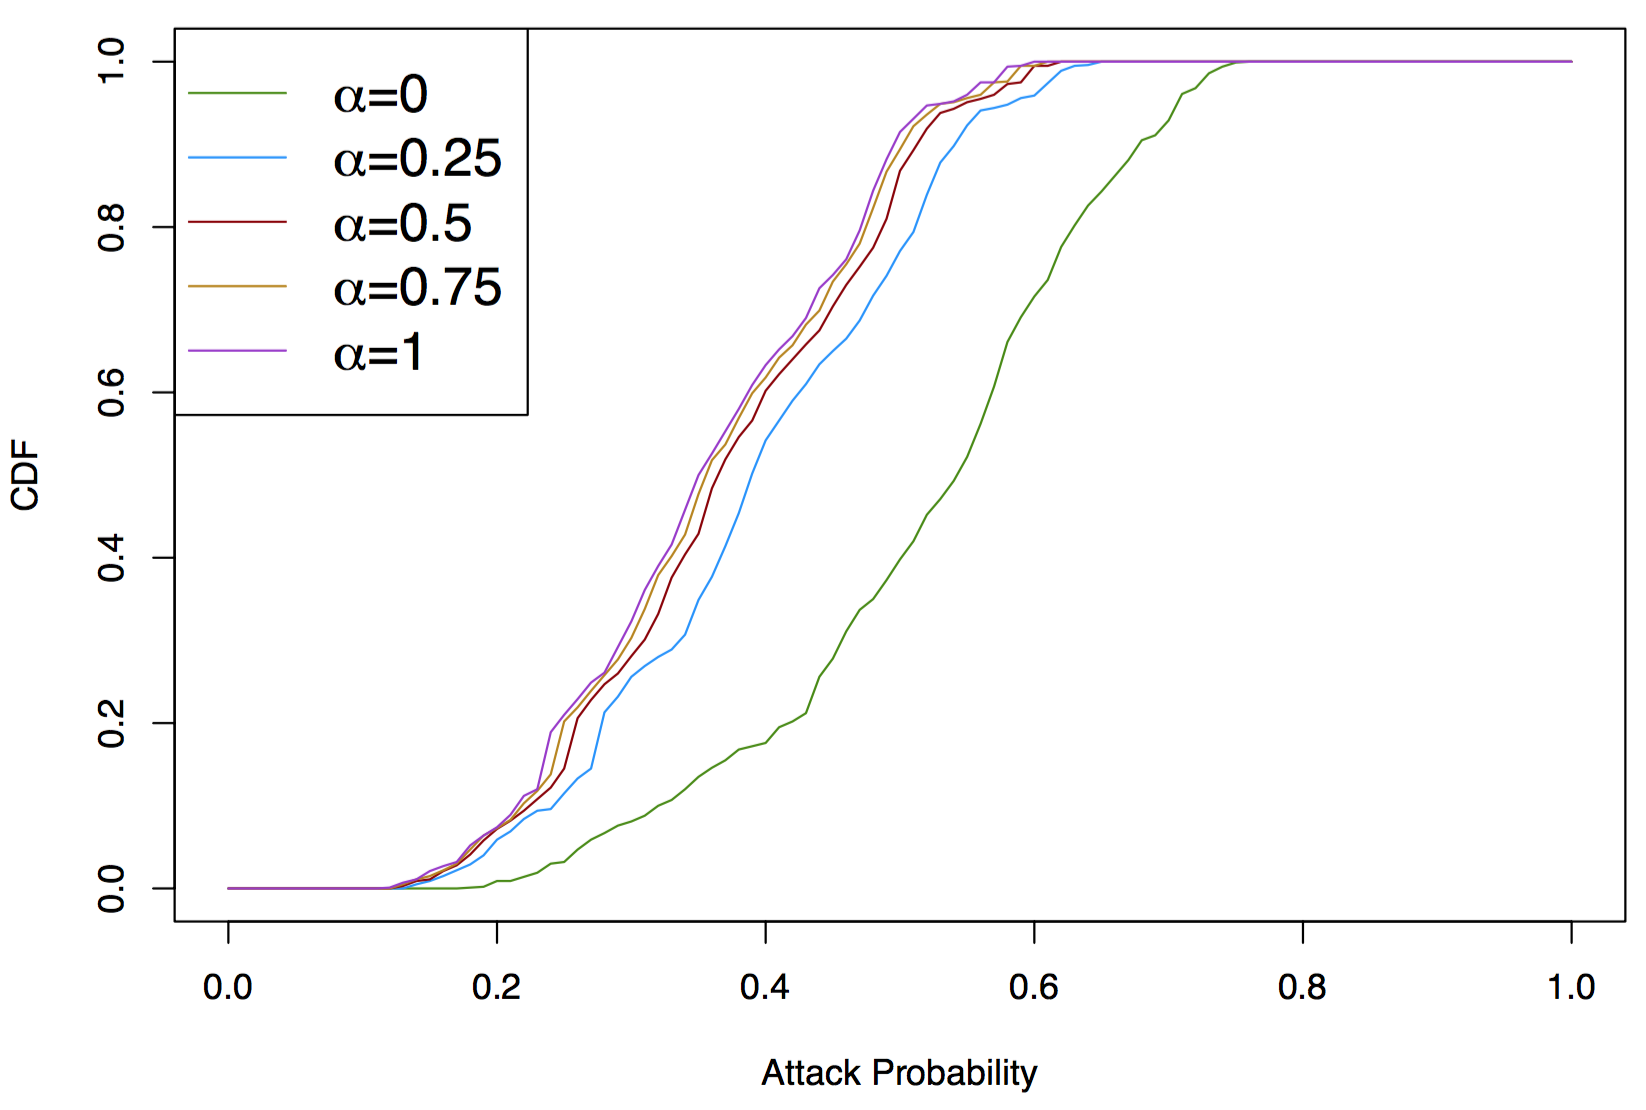
\includegraphics[width=80mm]{figure/attack}
\caption{Attack Probability with different $\alpha$ values \label{fig_attack}}
\end{figure}

We can see that $\alpha=1$ has the lowest probability of being affected by an attack, while its advantage to other $\alpha$ values is marginal. All of them have much lower probability compared to the bandwidth-only selection. 

We then evaluate it with random sampling of $g=10\%$ for $\alpha=\{0.25, 0.5\}$. Figure ~\ref{fig_attack_random} shows the result. Although there is a small increase in attack probability after the random sampling, it is still much lower than Vanilla Tor ($\alpha=0$). 

\begin{figure}[ht!]
\centering
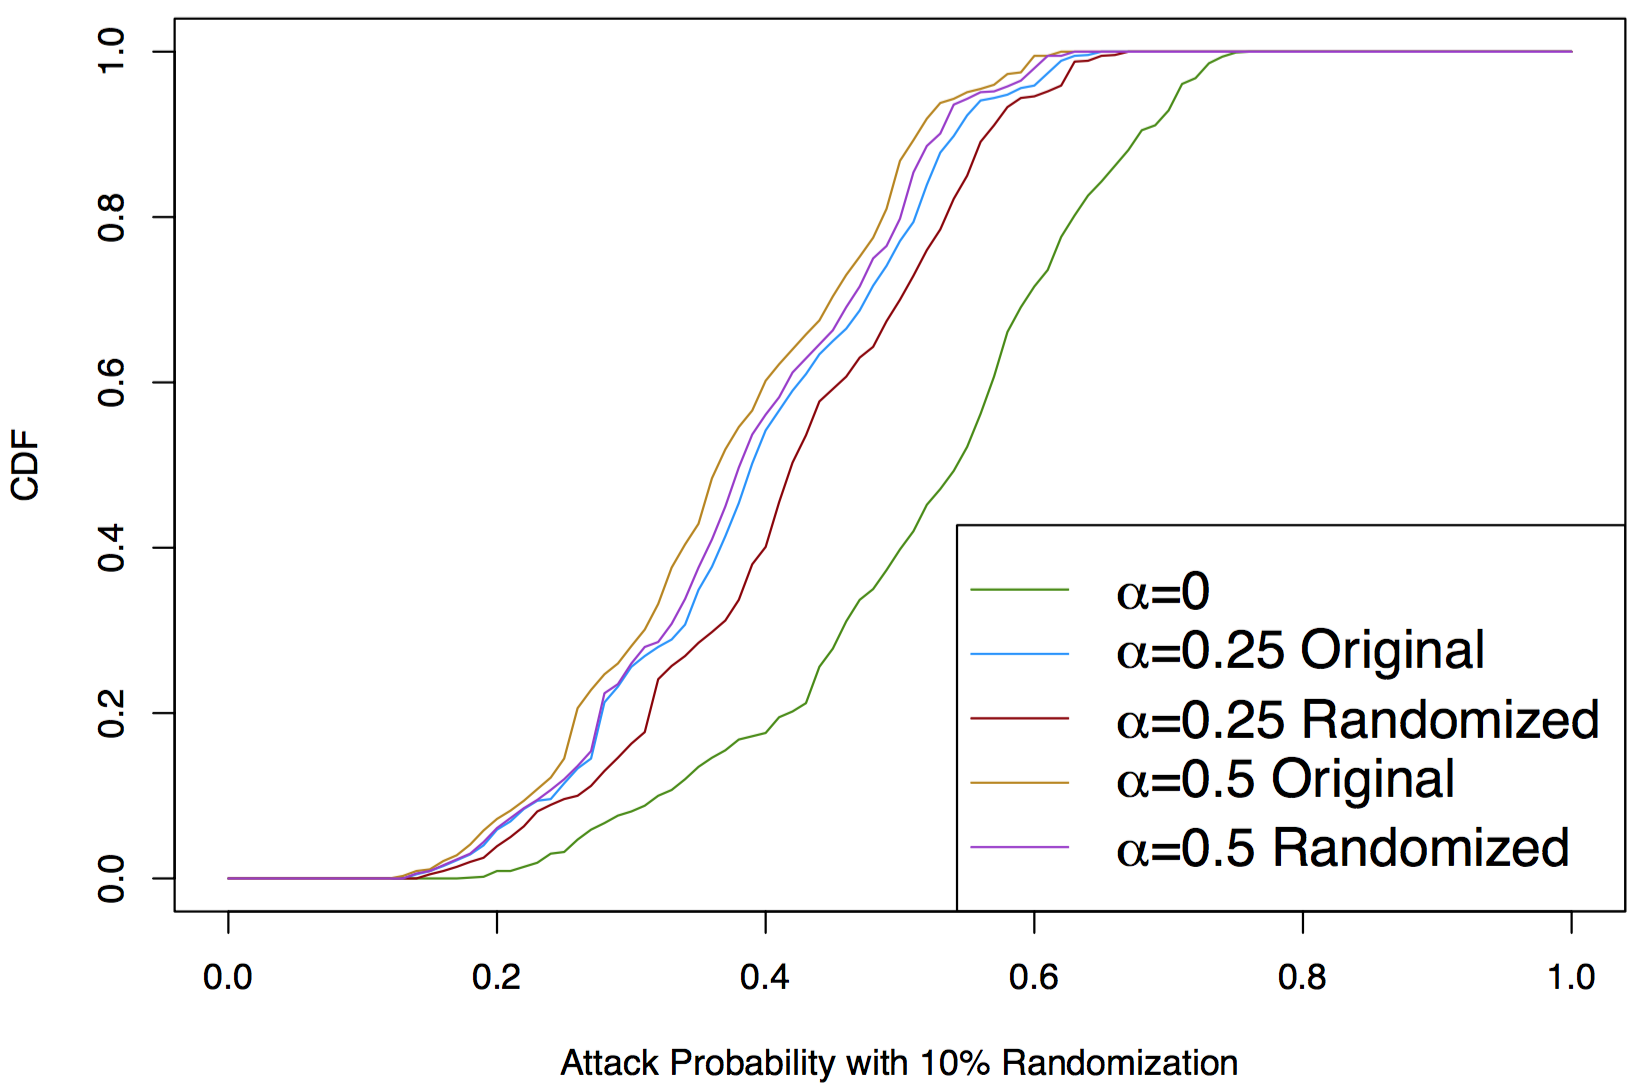
\includegraphics[width=80mm]{figure/attack_randomize}
\caption{Attack Probability with $g=10\%$ sampling \label{fig_attack_random}}
\end{figure}

\textbf{Relay selection variance} in entropy can be evaluated using Gini coefficient as the entropy evaluation metric, as it has been used in previous work to measure anonymity selection in Tor ~\cite{akhoondi2012lastor}. We first evaluate without  random sampling, for five values of $\alpha: \{0, 0.25, 0.5, 0.75, 1\}$ with $1000$ randomly selected ASes as source AS and Tor consensus data from January 2016. Figure ~\ref{fig_gini} shows the result. The green line to the right is when $\alpha = 0$, which is solely based on bandwidth resulting in a Gini coefficient of $0.51$ for all source ASes. The Gini coefficients for the other four $\alpha$ values which involve resilience-based selection are much lower than bandwidth-based selection, meaning that there is higher entropy and lower skew in probabilities of selecting any particular relay.

\begin{figure}[ht!]
\centering
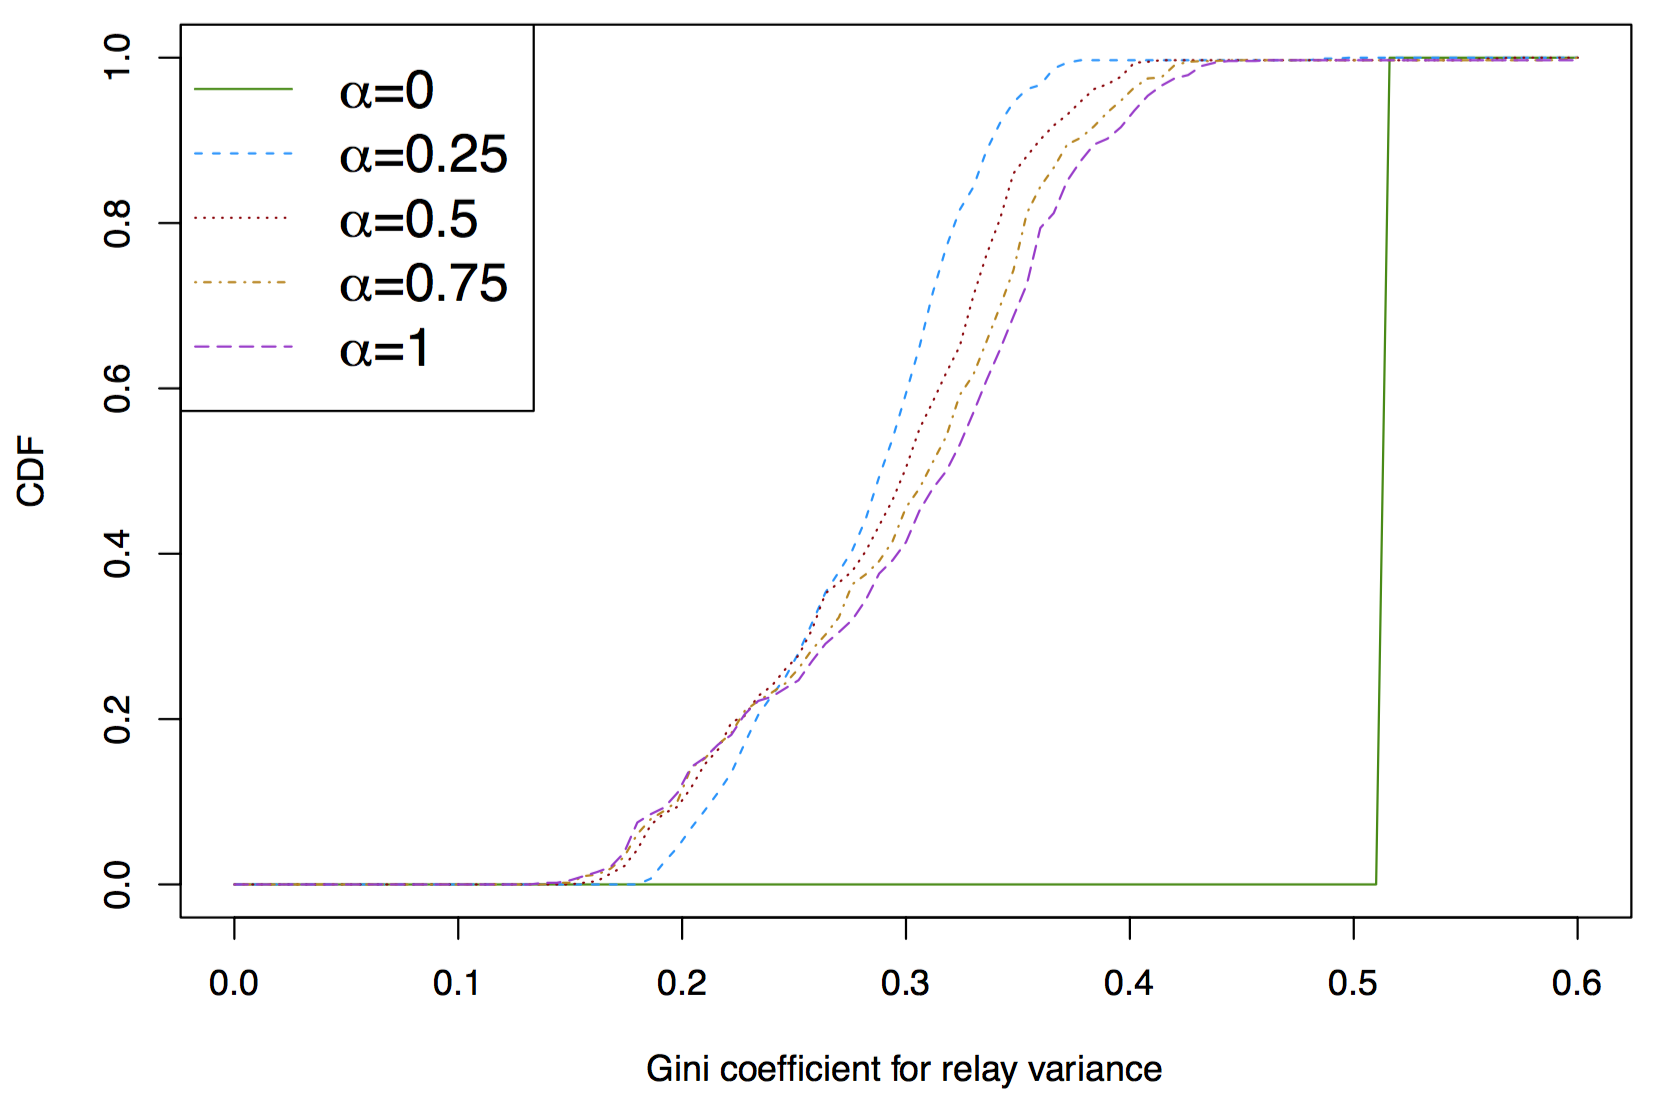
\includegraphics[width=80mm]{figure/gini_relay_variance}
\caption{Gini coefficients for relay variance given a client \label{fig_gini}}
\end{figure}

\begin{figure}[ht!]
\centering
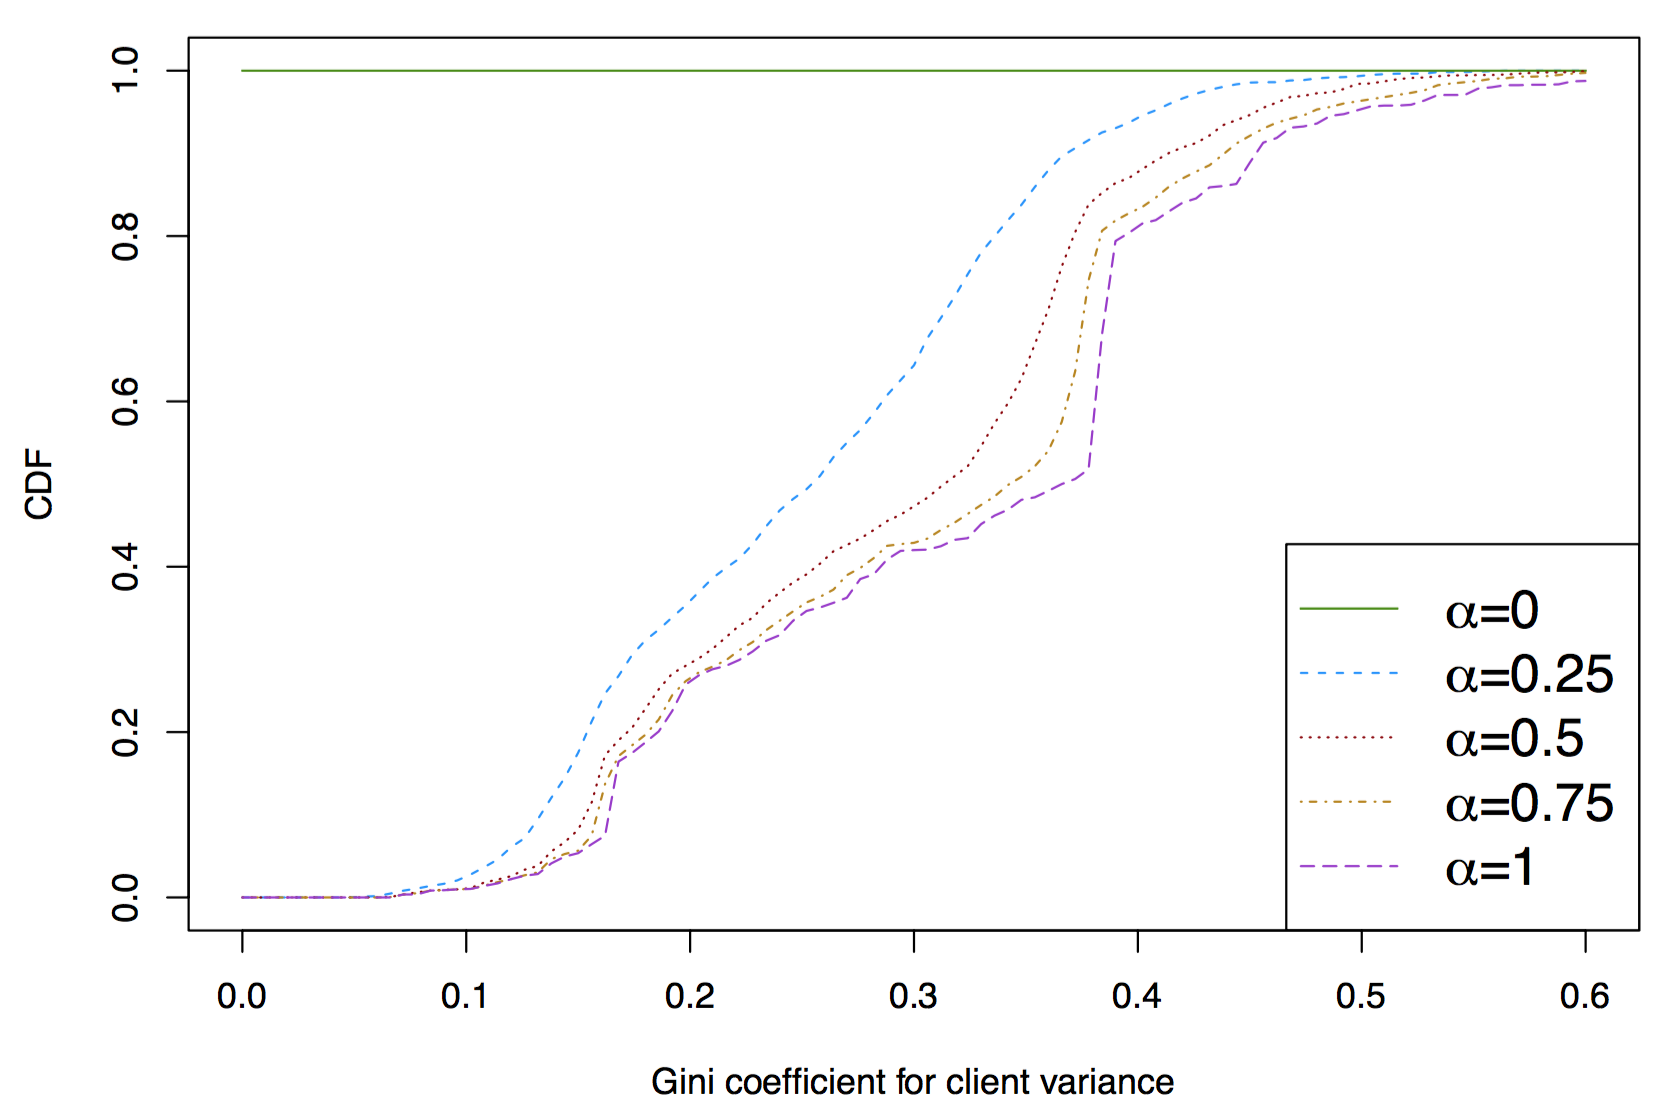
\includegraphics[width=80mm]{figure/gini_client_variance}
\caption{Gini coefficients for client variance given a relay \label{fig_gini_client}}
\end{figure}

Figure ~\ref{fig_gini_client} shows the Gini coefficient for the \emph{client} variance - probabilities of different Tor clients choosing a particular relay. The top line is bandwidth-only selection when $\alpha = 0$, and thus the probabilities of different clients choosing a relay are the same, resulting in Gini coefficient$=0$ for all relays. With resiliency-based selection, the skews in probabilities are higher. When $\alpha = 1$ (resiliency-only), $80\%$ of the relays have coefficients $> 0.4$. This skew in probability might be exploited by adversaries who can observe the client over a period of time to infer client locations given the differences in relay selection.

\begin{figure}[ht!]
\centering
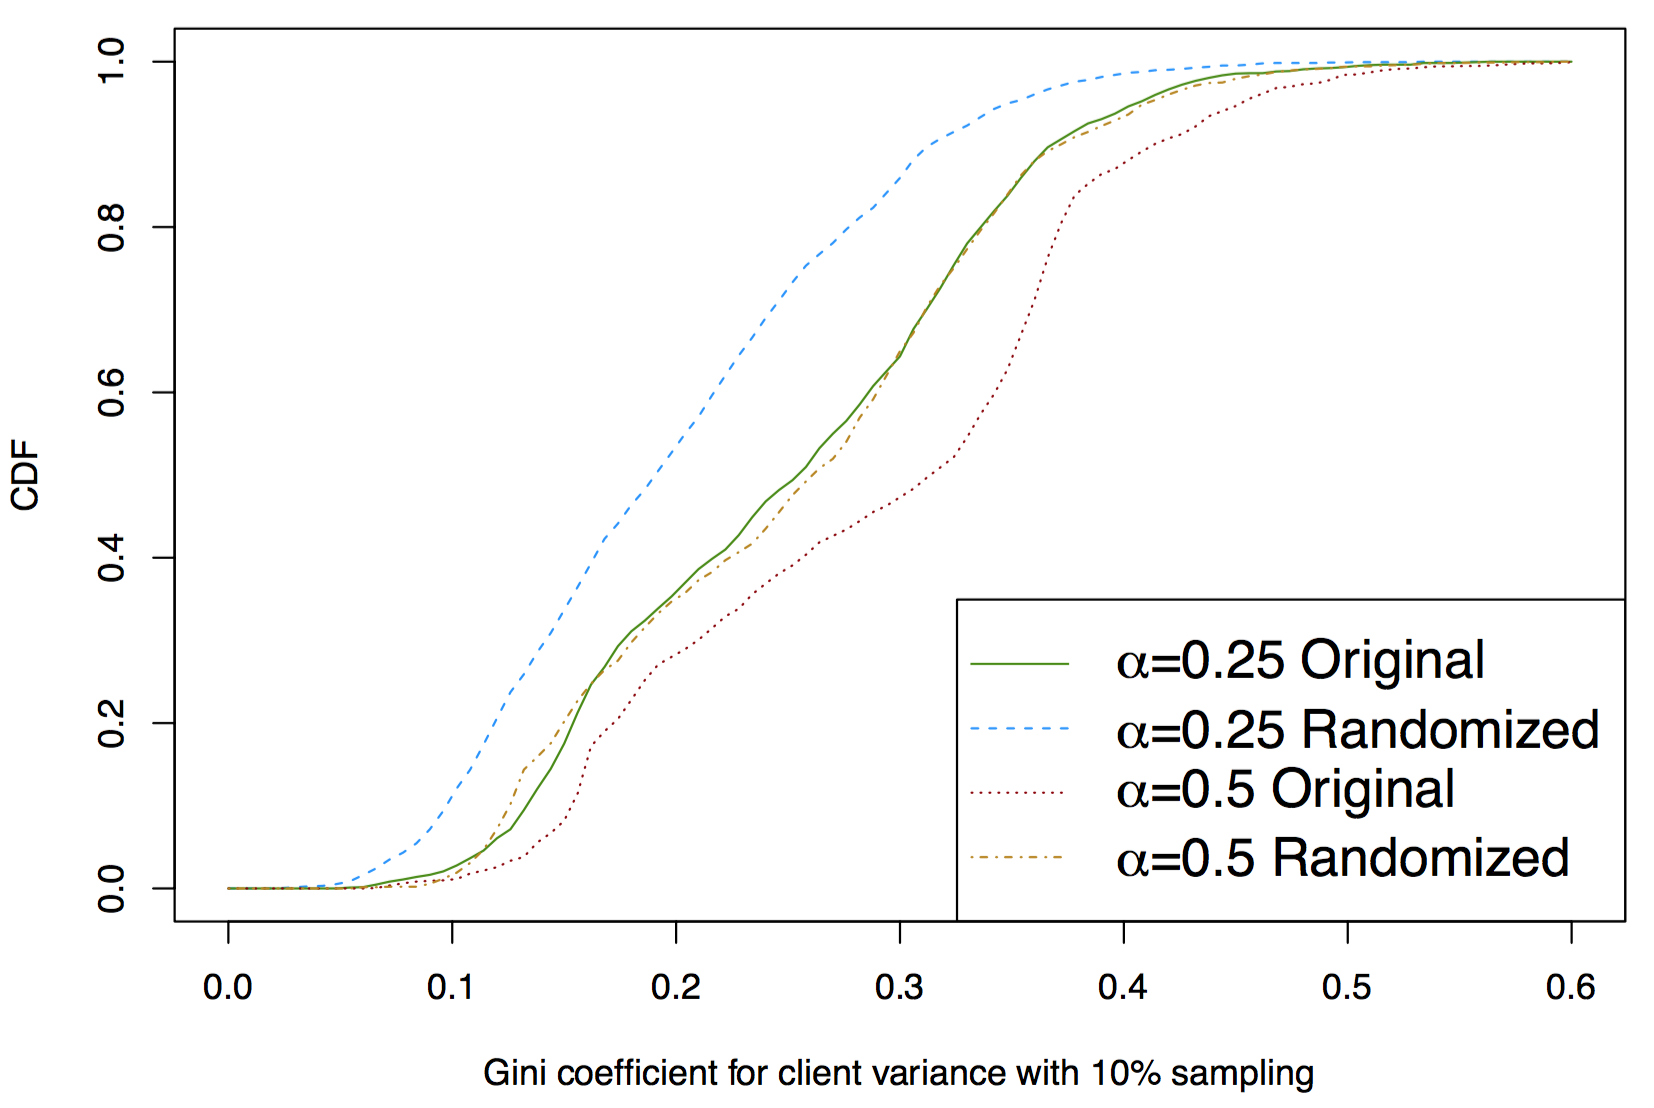
\includegraphics[width=80mm]{figure/randomize_client_gini}
\caption{Gini coefficients for client variance with $g=10\%$ sampling \label{fig_gini_client_random}}
\end{figure}

We then evaluate the Gini coefficient for client variance again with $g=10\%$ random sampling. Note that since $\alpha=\{0.75,1\}$ does not have a significant advantage in attack resiliency over $\alpha=\{0.25,0.5\}$ while resulting in higher skew in probabilities, so we focus on evaluating the later here. Figure ~\ref{fig_gini_client_random} shows that by performing $10\%$ random sampling, when $\alpha=0.25$, $80\%$ of the relays have coefficients reduced to $< 0.28$. Although this may still pose some vulnerability to client fingerprinting, we argue that since Tor clients only select guard relays at bootstrapping time, and would then use the same guard relays over several months or until the relays become unavailable, so fingerprinting the client could not be done in a reasonably short time, especially given the low variance of probabilities, as shown above.\\



\textbf{Formal anonymity assessment} of the relay selection algorithm is performed using MATor, a framework for assessing the degree of anonymity in Tor with rigorously proved anonymity bounds(citation here). We implemented our new relay selection algorithm into MATor source code, and evaluated in comparison with vanilla Tor. We used configuration of multiplicative factor$\epsilon=1.3$, ports setting of HTTPS+IRC vs. HTTPS, and for compromised nodes $0.5\%$ of total nodes. We evaluated using Tor consensus files from 2/1/2016 - 2/9/2016 and server descriptor from February 2016. Figure ~\ref{fig_mator} shows the result. 

\begin{figure}[ht!]
\centering
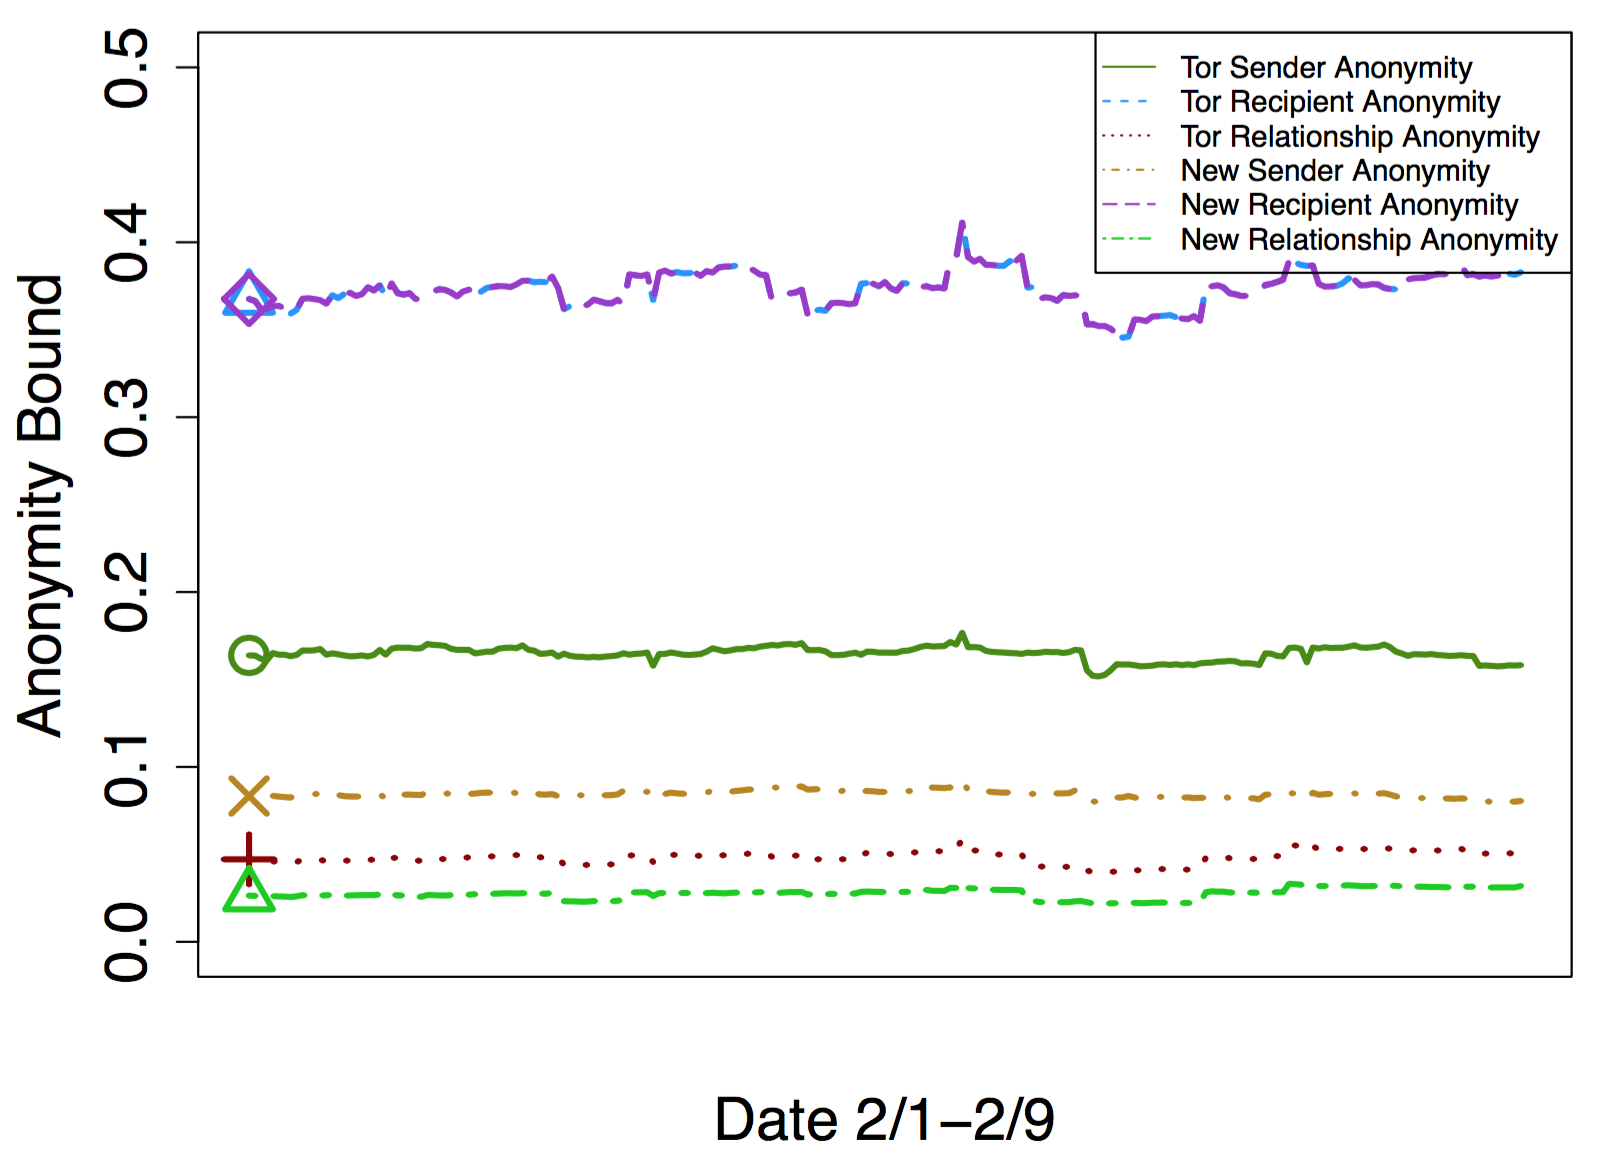
\includegraphics[width=80mm]{figure/mator}
\caption{MATor 2/1/2016 - 2/9/2016 (Ignore the numbers on x axis. I need to reformat this plot.) \label{fig_mator}}
\end{figure}

Our new guard relay selection has better (lower) anonymity bound on sender anonymity and relationship anonymity compared to current Tor path selection. Since we do not alter selection for exit relay, so recipient anonymity remains the same as vanilla Tor. 


%However, the variance in relay selection probability \emph{across} different source ASes is bigger than bandwidth-only: when $\alpha = 0$, all sources ASes have the same gini coefficient of $0.607$, while for other $\alpha$ values, the gini coefficient could vary from approximately $0.2$ to $0.4$, depending on the source AS. 



\subsubsection{Performance Evaluation}

First, we evaluate the runtime of the AS resilience calculation given a source AS. We pick $1000$ ASes randomly as the source AS, and record how much time it takes each of them to complete the calculation. Figure ~\ref{fig_ascal} show the CDF of the runtime of AS resilience calculation. Most of the source ASes finish within $0.6$ second. 

\begin{figure}[ht!]
\centering
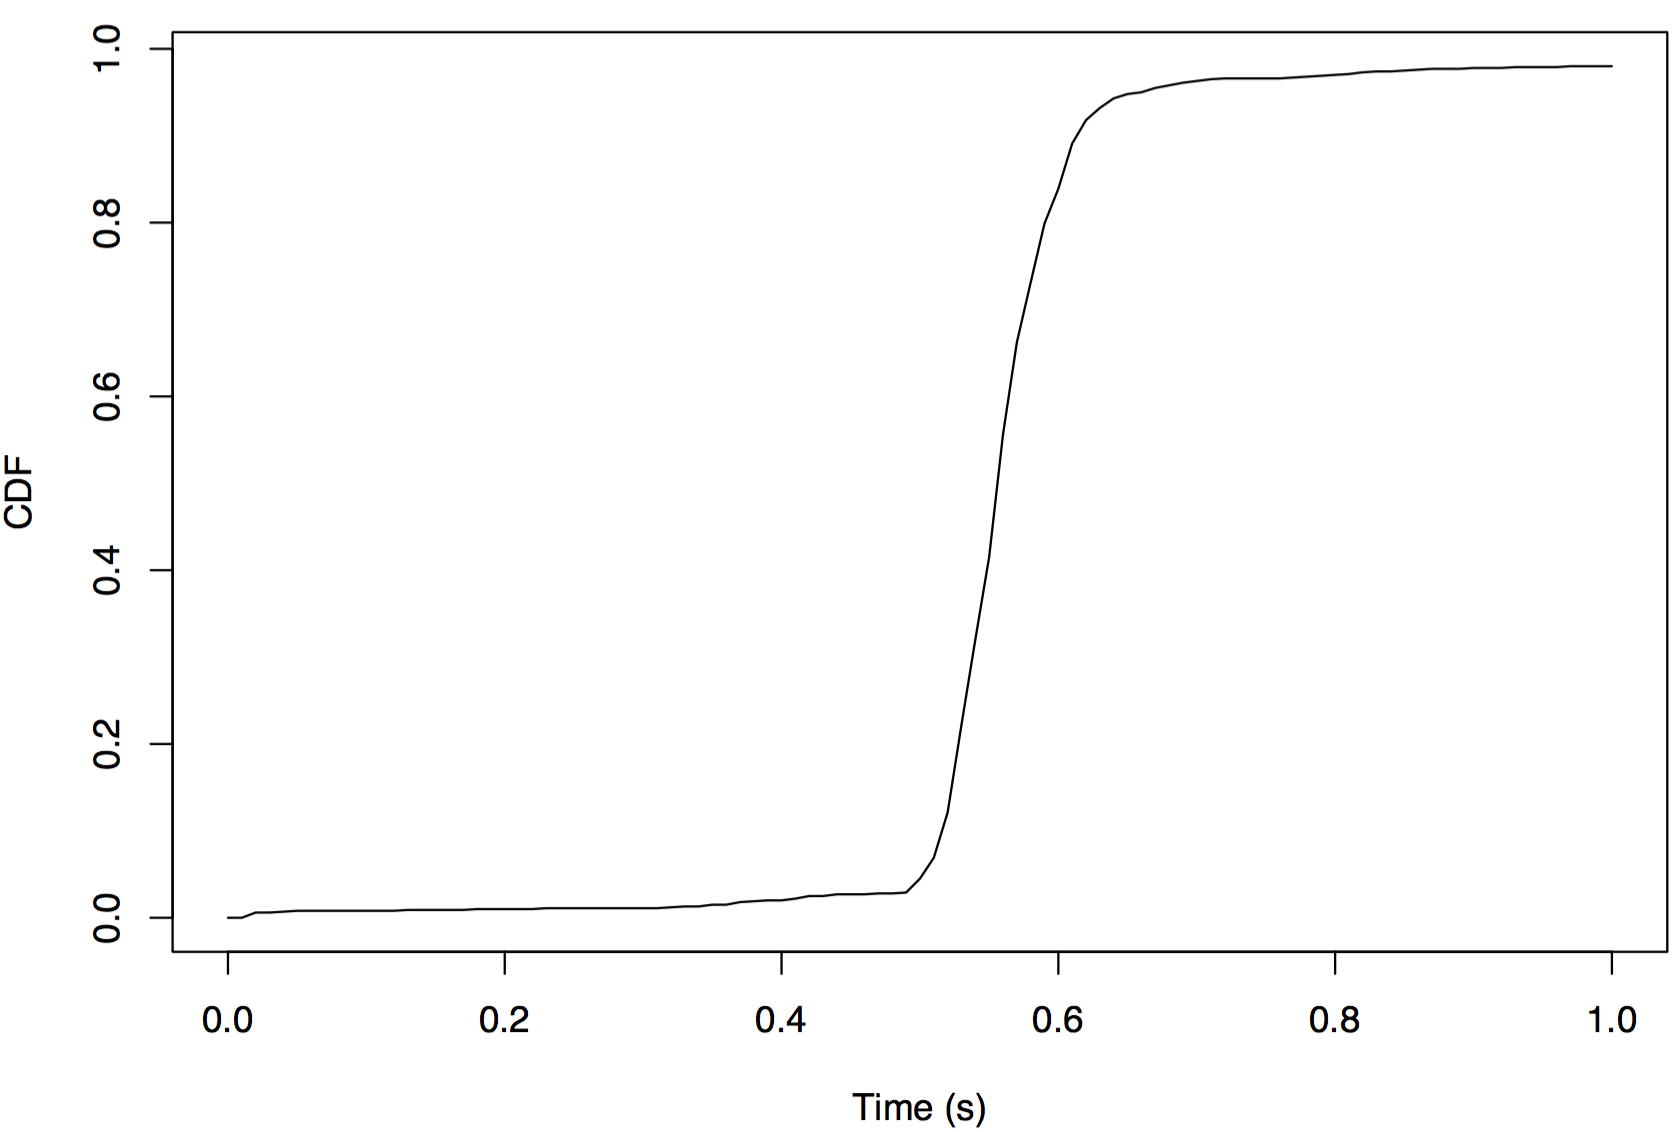
\includegraphics[width=80mm]{figure/runtime}
\caption{Runtime of AS resilience calculation from a given source AS \label{fig_ascal}}
\end{figure}

Next, we installed our new Tor client on $26$ Planetlab nodes located in different ASes, and performed page loads of Alexa top 100 websites. We compared the performance of $\alpha={0.25,0.5}$ with $g=10\%$ random sampling against vanilla Tor. Figure ~\ref{fig_pageload} shows the page load time, and all have almost the same performance. This shows that we do not have any performance loss by using our new relay selection algorithm. 

\begin{figure}[ht!]
\centering
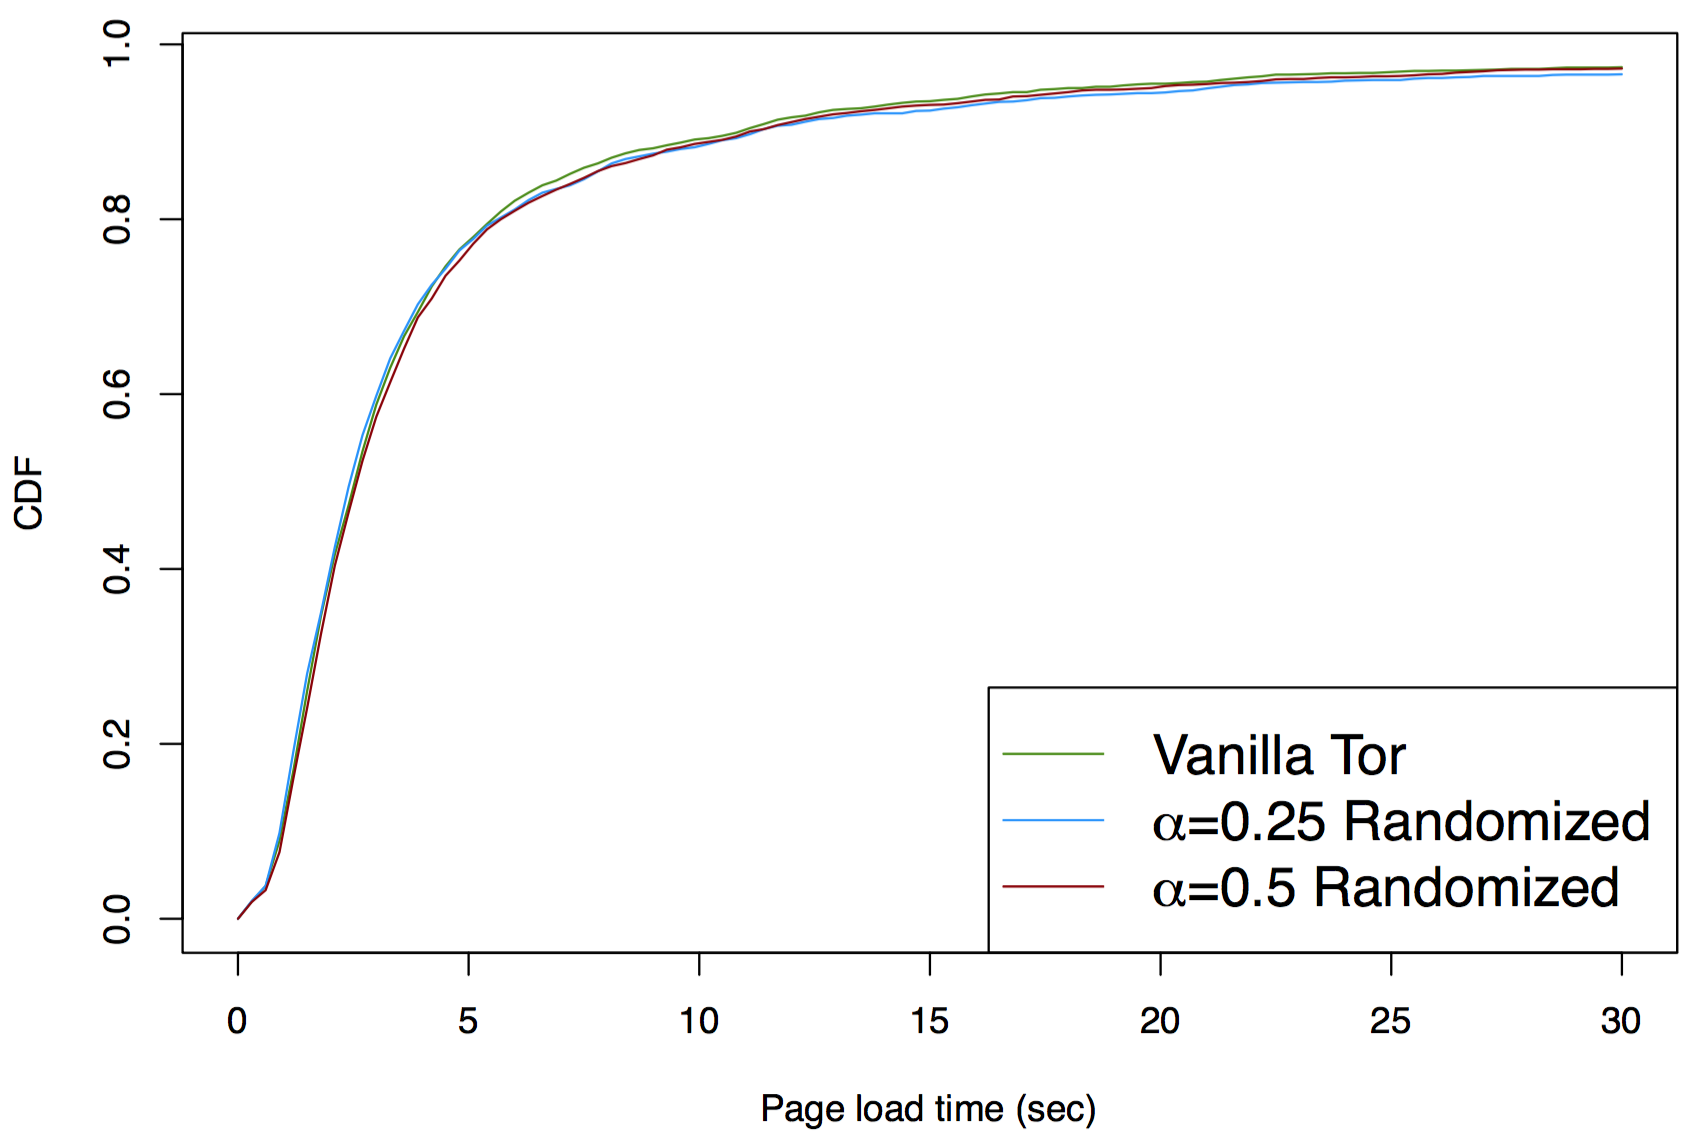
\includegraphics[width=80mm]{figure/pageloadtime}
\caption{Page load time of Alexa top 100 sites \label{fig_pageload}}
\end{figure}



